%\documentclass[a0,portrait]{a0poster}
\documentclass[a0,landscape]{a0poster}
\pagestyle{empty}
\setcounter{secnumdepth}{0}
\usepackage[absolute]{textpos}
\usepackage{graphicx}
\usepackage{times}
\usepackage{fancybox}
\usepackage{color}
\usepackage{url}
\usepackage{amsmath}
\usepackage{amsfonts}
\usepackage{esint}
\usepackage{sidecap}
%\usepackage{algorithmic}
\usepackage{tabularx}
\usepackage{pifont}
\usepackage{natbib}

\usepackage{hyperref}
\usepackage{caption}
\usepackage{subcaption}
% \usepackage{pdfpages}  # causes an error, and we don't even generate a multi-page document
\usepackage{amsmath, amsthm, amssymb}
\DeclareMathOperator{\Tr}{Tr}
\usepackage{algpseudocode}
\usepackage{algorithm}
\usepackage{float}
\usepackage{hyperref}
\usepackage{textcomp}

\newtheorem{proposition}{Proposition}
\newtheorem{corollary}{Corollary}
\newtheorem{theorem}{Theorem}


\definecolor{DarkBlue}{rgb}{0.4,0.4,1}
\definecolor{Red}{rgb}{0.9,0.0,0.1}
\definecolor{Black}{rgb}{0.0,0.0,0.0}
\definecolor{Green}{rgb}{0.0,0.9,0.1}
%\definecolor{Gray}{rgb}{0.9,0.9,0.9}
%\definecolor{mycolor}{RGB}{220,220,240}
\definecolor{MilaBlue}{RGB}{78,179,225} % lighter, PMS 306
%\definecolor{MilaBlue}{RGB}{35,154,204} % darker, PMS 639
\definecolor{OppositeOrange1}{RGB}{255,129,0}

\def\CRed#1{{\color{Red}{#1}}}
\def\CBlue#1{{\color{DarkBlue}{#1}}}
\def\CGreen#1{{\color{Green}{#1}}}

\let\Textsize\normalsize
\def\Head#1{\begin{center}\noindent{\LARGE\bf\color{MilaBlue}#1}\end{center}\bigskip}
\def\LHead#1{\noindent{\LARGE\color{MilaBlue} #1}\smallskip}
\def\Subhead#1{\begin{center}\noindent{\large\color{Black}#1}\end{center}\smallskip}
%\def\Title#1{\noindent{\Huge\bf\color{OppositeOrange1} #1}}
\def\Title#1{\noindent{\Huge\bf\color{Black} #1}}

\TPGrid[25mm,20mm]{114}{80}  % 1 unit ~ 1 cm
%\TPGrid[25mm,20mm]{79}{115}  % 1 unit ~ 1 cm
\parindent=0pt
%\parskip=2.0\baselineskip

% try to have more space between lines by
% calling \onehalfspacing after the heading
% of the poster
\usepackage{setspace}

\makeatother

%%%%%%%%%%%%%%%%%%%%%%%%%%%%%%%%%%%%%%%
\begin{document}


%%%%%%%%%%%%%%%%%%%%%%%%%%%%%%%%%%%%%%%%%%%%%%%%%%%%%%%%%%%%%%%%%%%%%%%%%%
%%% HEADER
%%%%%%%%%%%%%%%%%%%%%%%%%%%%%%%%%%%%%%%%%%%%%%%%%%%%%%%%%%%%%%%%%%%%%%%%%%

% with a rough white border [trim = 100mm 95mm 100mm 80mm, clip, width=40cm]
% as tight as possible [trim = 106mm 97mm 113mm 81mm, clip, width=40cm]
\begin{textblock}{10}(3,-0.5)
\scalebox{0.5}{
\includegraphics[trim = 106mm 97mm 113mm 81mm, clip, width=30cm]{MILA_umontreal_20160314.pdf}}
\end{textblock}

\begin{textblock}{114}(-1,-1)
  \begin{center}
    \hspace{2cm}
    \begin{minipage}{114cm}
      \baselineskip=3\baselineskip
      \Title{\begin{center}Active Reinforcement Learning: Observing Rewards at a Cost \end{center}}
      \vspace{-1cm}
      \LHead{\begin{center}
          David Krueger \hspace{2cm} Jan Leike \hspace{2cm} John Salvatier \hspace{2cm} Owain Evans
      \end{center}}
      \vspace{-2cm}
    \end{minipage}
    \hspace{2cm}
  \end{center}
\end{textblock}

\onehalfspacing

\begin{textblock}{150}(3,-0.5)
%\scalebox{0.5}{
\includegraphics[trim = 106mm 97mm 113mm 81mm, clip, width=30cm]{FHI.pdf}}
\hspace{92cm}
\scalebox{0.9}{
\includegraphics{FHI.pdf}}
\end{textblock}

% TITLE BAR
\begin{textblock}{120}(-4,9)
{\color{MilaBlue}{\vrule depth 0pt height 0.5cm width 125cm}}
\end{textblock}

%%%%%%%%%%%%%%%%%%%%%%%%%%%%%%%%%%%%%%%%%%%%%%%%%%%%%%%%%%%%%%%%%%%%%%%%%%
%%% Block prototype
%%%%%%%%%%%%%%%%%%%%%%%%%%%%%%%%%%%%%%%%%%%%%%%%%%%%%%%%%%%%%%%%%%%%%%%%%%

%\begin{textblock}{0}(x,y)
%% x, y are in approximate centimeters, x should be one of {-1, 40}
%\Ovalbox{\hspace{0.5cm}
%\begin{minipage}{38cm} %\vspace{0.5cm}
%\Head{Title}
%
%Text
%
%\vspace{0.5cm}
%\end{minipage}
%\hspace{0.5cm}}
%\end{textblock}


%%%%%%%%%%%%%%%%%%%%%%%%%%%%%%%%%%%%%%%%%%%%%%%%%%%%%%%%%%%%%%%%%%%%%%%%%%
%%% FIRST COLUMN
%%%%%%%%%%%%%%%%%%%%%%%%%%%%%%%%%%%%%%%%%%%%%%%%%%%%%%%%%%%%%%%%%%%%%%%%%%

\begin{textblock}{0}(-1,12)

\begin{minipage}{35cm}
\Head{What is Active RL?}

\end{minipage}
\end{textblock}


\begin{textblock}{0}(-1,34)
\begin{minipage}{35cm}
\Head{Motivations}

\begin{itemize}
\item
\end{itemize}

\end{minipage}
\end{textblock}

%%%%%%%%%%%%%%%%%%%%%%%%%%%%%%%%%%%%%%%%%%%%%%%%%%%%%%%%%%%%%%%%%%%%%%%%%%
%%% SECOND COLUMN
%%%%%%%%%%%%%%%%%%%%%%%%%%%%%%%%%%%%%%%%%%%%%%%%%%%%%%%%%%%%%%%%%%%%%%%%%%

%%%%%%%%%%%%%%%%%%%


\begin{textblock}{0}(38, 12)
\begin{minipage}{35cm}
\Head{MDP Algorithms}
\end{minipage}
\end{textblock}

%%%%%%%%%%%%%%%%%%%
\begin{textblock}{0}(38,38)
\begin{minipage}{35cm}
\Head{Bandit Algorithms}
\end{minipage}
\end{textblock}

%%%%%%%%%%%%%%%%%%%
\begin{textblock}{0}(38,54)
\begin{minipage}{35cm}
\Head{Bandit Experiments}
\end{minipage}
\end{textblock}


%%%%%%%%%%%%%%%%%%%%%%%%%%%%%%%%%%%%%%%%%%%%%%%%%%%%%%%%%%%%%%%%%%%%%%%%%%
%%% THIRD COLUMN
%%%%%%%%%%%%%%%%%%%%%%%%%%%%%%%%%%%%%%%%%%%%%%%%%%%%%%%%%%%%%%%%%%%%%%%%%%

% TODO: mention that our algorithms either search "equivalently" or "independently" (some combination seems appropriate...)

\begin{textblock}{0}(77,12)
\begin{minipage}{35cm}
\Head{MDP Environments}
% TODO: other example environments (e.g. two-state moat)
% TODO: captions
\iffalse
\begin{center}
    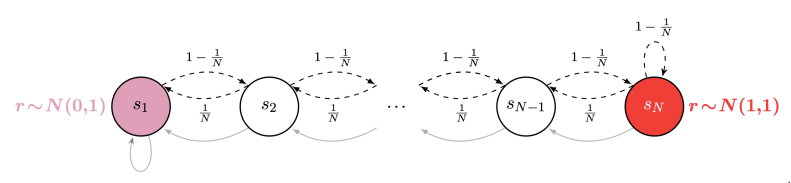
\includegraphics[width=\textwidth]{chain_figure.png}
    %train loss, learning rate $0.01$
    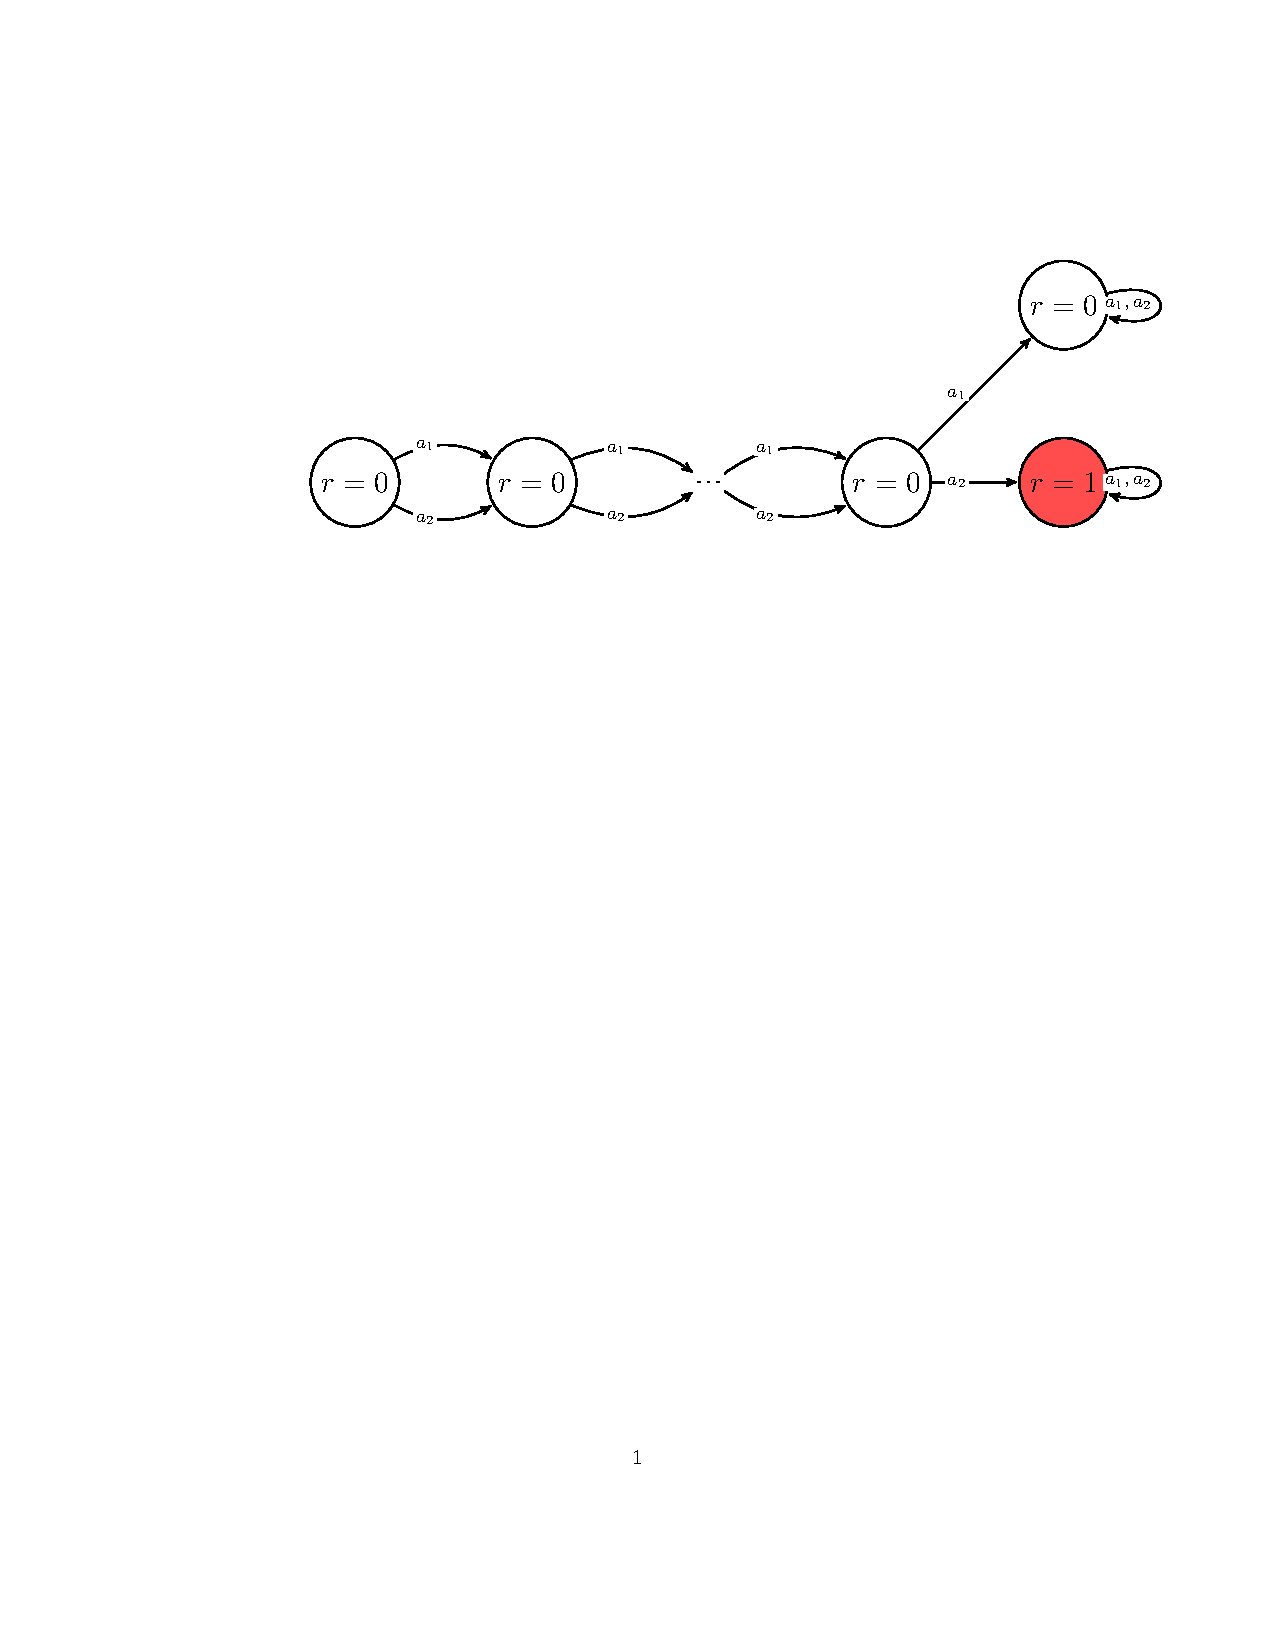
\includegraphics[width=\textwidth]{long-y.pdf}
    %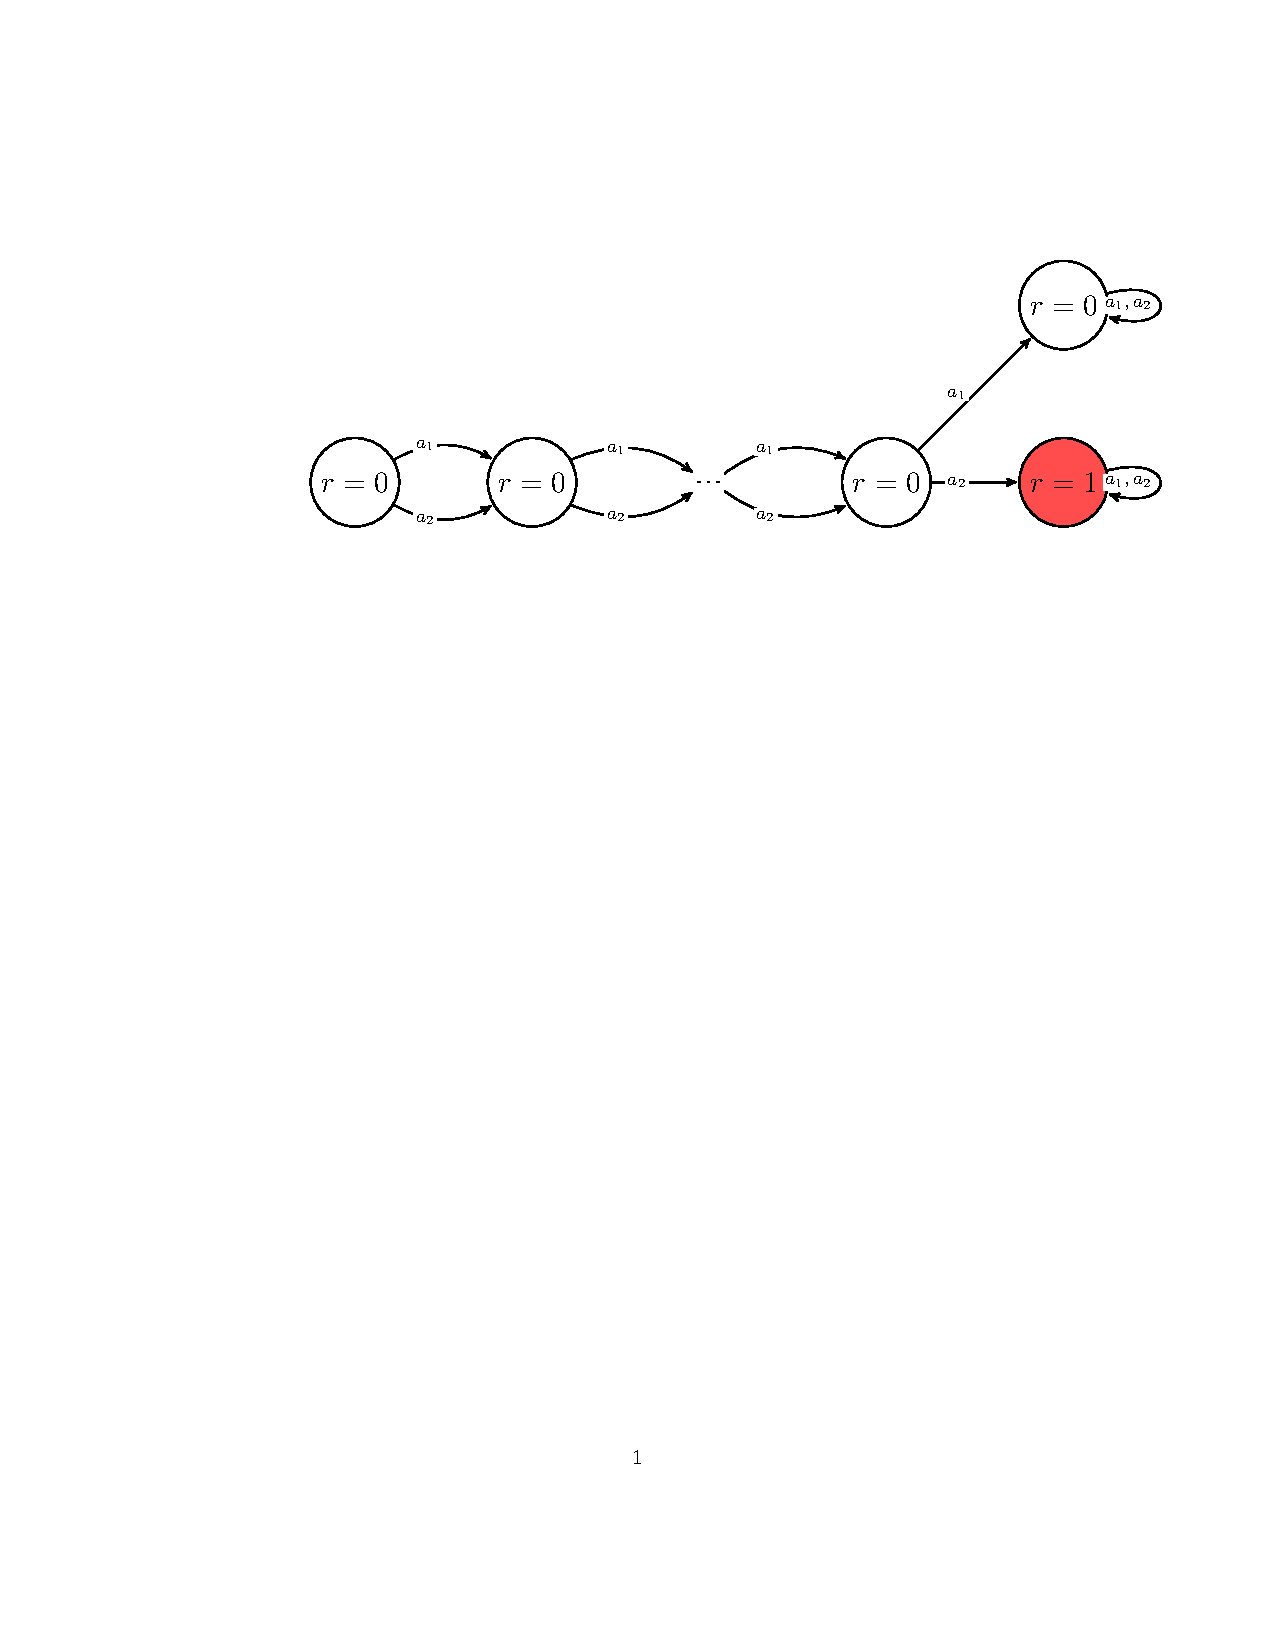
\includegraphics[trim = 106mm 97mm 113mm 81mm, clip, width=32cm]{long-y.pdf}
    %train loss, learning rate $0.001$
\end{center}
\fi

\end{minipage}
\end{textblock}


\begin{textblock}{0}(77,54)
\begin{minipage}{35cm}
\Head{MDP Experiments}
\end{minipage}
\end{textblock}


% ACKNOWLEDGEMENTS
\begin{textblock}{0}(77,68)
\begin{minipage}{35cm}
\vspace{0.5cm}
\small{%tiny
\bibliography{strings,strings-short,aigaion-short,ml}
\bibliographystyle{natbib}
}
\vspace{2em}
This work was supported by Future of Life Institute grant 2015-144846 (JS, DK, OE). 
We thank Andreas Stuhlm\"uller, Tor Lattimore, Reimar Leike, Ryan Lowe, Akram Erraqabi, and Jessica Taylor for helpful discussions.
The authors acknowledge the use of the University of Oxford Advanced Research Computing (ARC) facility in carrying out this work. 
\end{minipage}

\vspace{0.5cm}
\hspace{0.5cm}
\end{textblock}
\end{document}
